%
% File acl2017.tex
%
%% Based on the style files for ACL-2015, with some improvements
%%  taken from the NAACL-2016 style
%% Based on the style files for ACL-2014, which were, in turn,
%% based on ACL-2013, ACL-2012, ACL-2011, ACL-2010, ACL-IJCNLP-2009,
%% EACL-2009, IJCNLP-2008...
%% Based on the style files for EACL 2006 by 
%%e.agirre@ehu.es or Sergi.Balari@uab.es
%% and that of ACL 08 by Joakim Nivre and Noah Smith

\documentclass[11pt,a4paper]{article}
\usepackage[hyperref]{acl2017}
\usepackage{times}
\usepackage{latexsym}
\usepackage{graphicx}
\usepackage{amsmath}
\usepackage{amssymb}
\usepackage{url}

\aclfinalcopy % Uncomment this line for the final submission
%\def\aclpaperid{***} %  Enter the acl Paper ID here

%\setlength\titlebox{5cm}
% You can expand the titlebox if you need extra space
% to show all the authors. Please do not make the titlebox
% smaller than 5cm (the original size); we will check this
% in the camera-ready version and ask you to change it back.

% \newcommand\BibTeX{B{\sc ib}\TeX}

\title{Neural Knowledge Acquisition via Joint Representation of Knowledge Graph and Text}

% \author{First Author \\
%   Affiliation / Address line 1 \\
%   Affiliation / Address line 2 \\
%   Affiliation / Address line 3 \\
%   {\tt email@domain} \\\And
%   Second Author \\
%   Affiliation / Address line 1 \\
%   Affiliation / Address line 2 \\
%   Affiliation / Address line 3 \\
%   {\tt email@domain} \\}

% \date{}

\begin{document}
\maketitle

\begin{abstract}
   In this paper, we propose a novel joint representation learning framework for knowledge acquisition on two tasks, knowledge graph completion (KGC) and relation extraction (RE) from text. The joint learning mechanism enables us to take both knowledge graphs (KGs) and text into consideration and perform better KGC and RE. In this framework, representations of KGs and text are learned within a unified semantic space and share parameters via alignments between KGs and text. Due to the joint mechanism, structural KG features and flexible textual features are successfully incorporated together to enhance the representations. In experiments, we evaluate our joint model on relation extraction, entity prediction and relation prediction, and the results show that our joint model can significantly and consistently improve the performance as compared with other baselines. 
\end{abstract}


\section{Introduction}
\label{intro}

People construct various large-scale knowledge graphs (KGs) to organize structural knowledge about the world, such as WordNet \cite{miller1995wordnet}, YAGO \cite{suchanek2007yago}, DBPedia \cite{auer2007dbpedia}, Freebase \cite{bollacker2008freebase}, Knowledge Vault \cite{dong2014knowledge} and Wikidata \cite{vrandevcic2014wikidata}. A typical knowledge graph is a multiple-relational directed graph with nodes corresponding to entities, and edges corresponding to relations between these entities. The facts in KGs are usually recorded as a set of relational triples ($h$, $r$, $t$) with $h$, $t$ indicating \emph{head}, \emph{tail} entities and $r$ indicating the relation between $h$ and $t$, e.g., (\emph{Mark Twain}, \texttt{PlaceOfBirth}, \emph{Florida}). Because of rich structural information, KGs are playing an important role in many applications such as question answering and web search.

\begin{figure}[]
\centering
\includegraphics[width=\columnwidth]{joint.jpg}
\caption{The framework for joint representation learning of the knowledge graph and text.}
\label{fig:joinglearning}
\end{figure}

However, most large-scale KGs are usually far from complete. There are typically two tasks to extend KGs, knowledge graph completion (KGC) and relation extraction (RE) from text. KGC aims to enrich KGs with novel facts, based on the network structure of KGs. Many graph-based methods have been proposed to mine novel facts \cite{lao2011random,lao2010relational}. In recent years, neural-based knowledge representation methods have been proposed to encode both entities and relations into a low-dimensional space, which are able to find novel facts \cite{bordes2013translating,wang2014transh,lin2015learning,ji2015knowledge,he2015learning,xiao2015transg,ji2016knowledge}. 

RE aims to extract relational facts from plain text. Many efforts are also devoted to do this \cite{surdeanu2012multi,riedel2013relation,min2013distant,zeng2014relation,zeng2015distant,lin2016neural,zeng2016incorporating}. The two tasks are closely relevant. However, most conventional methods haven't performed knowledge acquisition by jointly considering KGs and text.


% the past approaches seldom solve them at the same time by jointly considering KGs and text.

Some pioneering works have explored to fuse KGs and text. For example, \newcite{wang2014knowledge} performs joint learning by simply aligning words in text and entities in KGs. Then, \newcite{xie2016representation,wu2016knowledge} encode text descriptions to enhance entity embeddings, and \newcite{toutanova2015representing} extracts textual relations from plain text using dependency parsing to enhance relation embeddings. These works either consider only partial information in text (just entity mentions or textual relations), or rely on complicated linguistic analysis (e.g. dependency parsing) which may bring inevitable parsing errors.

To address these issues, we propose a novel framework for joint representation learning. As shown in Figure \ref{fig:joinglearning}, the framework is expected to take advantages of both KGs and text via comprehensive alignments with respect to words, entities and relations. Moreover, our method applies deep neural networks with a knowledge-based attention mechanism instead of conventional linguistic analysis to encode the semantics of sentences, which is especially capable of modeling large-scale and noisy Web text. 

We conduct experiments on a real-world dataset whose KG is extracted from Freebase and text is derived from the New York Times corpus. We evaluate our method on both KGC (entity prediction and relation prediction) and RE (relation extraction from text). Experimental results demonstrate that, our method can effectively perform joint representation learning and obtain more informative knowledge and text representation, which significantly outperforms other baseline methods in knowledge acquisition from either KGs or text.

\section{Related Work}
\label{sec:related}
Our work relates to representation learning of KGs, textual relations, and neural networks with attention. Related works are reviewed as follows.

\textbf{Representation Learning of KGs.} A variety of approaches have been proposed to encode both entities and relations into a continuous low-dimensional space. TransE \cite{bordes2013translating} regards the relation $r$ in each fact ($h$, $r$, $t$) as a translation from $h$ to $t$ within the low-dimensional space, i.e., $\textbf{h} + \textbf{r} = \textbf{t}$, where $\textbf{h}$ and $\textbf{t}$ are entity embeddings and $\textbf{r}$ is relation embedding. Despite of its simplicity, TransE achieves the amazing performance for KG representation. Many recent models are extended from TransE.

In this paper, we simply incorporate TransE in our method to handle representation learning of KGs. Note that, our method is also flexible to incorporate extension models of TransE, such as TransH \cite{wang2014transh}, TransR \cite{lin2015learning}, TransD \cite{ji2015knowledge} and TranSparse \cite{ji2016knowledge}, which is not the focus of this paper and will be explored in our future work.

% \textbf{Representation Learning of Words.} Given a text corpus, we can learn word representations without supervision. Continuous Bag-of-Words (CBOW) \cite{mikolov2013efficient} and Skip-Gram \cite{mikolov2013efficient} are universal methods for word representation learning. As reported in many previous works, being initialized with pre-trained word embeddings will significantly benefit deep neural network. In this work, we apply Skip-Gram for word representation learning.

\textbf{Representation Learning of Textual Relations.} Many works aim to extract relational facts from large-scale text corpora \cite{mintz2009distant,riedel2010modeling}. In recent years, deep neural models such as convolutional neural networks (CNN) \cite{zeng2014relation,zeng2015distant,lin2016neural}, recurrent neural networks (RNN) \cite{zhang2015relation} and long-short term memory networks (LSTM) \cite{xu2015classifying,miwa2016end} have been proposed to encode semantics of sentences, and identify relations between entities in the given sentences. As compared to conventional models, neural models are capable of accurately capturing textual relations without explicit linguistic analysis. In this paper, we apply CNN to embed textual relations due to its time efficiency.

\textbf{Neural Networks with Attention.} The attention mechanism is implemented to select the most relevant and important hidden features in text, which is first incoporated in neural networks for machine translation by \newcite{bahdanau2014neural}. The mechanism has also been used in various NLP tasks, such as entity type classification \cite{shimaoka2016attentive}, machine reading \cite{dhingra2016gated,sordoni2016iterative} and relation extraction \cite{lin2016neural}. In this paper, we propose a knowledge-based attention mechanism for sentence encoding. Different from conventional attention mechanisms use the fuzzy information from text, our knowledge-based attention use the discriminative information from KGs to highlight important components for representation learning, which is more efficient.


\section{The Framework}
In this section we introduce the framework of joint representation learning, starting with notations and definitions.

\subsection{Notations and Definitions}

We denote a knowledge graph as $G = \{E, R, T\}$, where $E$ indicates a set of entities, $R$ indicates a set of relation types, and $T$ indicates a set of fact triples. Each triple $(h, r, t) \in T$ indicates there is a relation $r \in R$ between $h \in E$ and $t \in E$.

Accompanying with $G$, we denote a text corpus as $D$, which is consisting of sentences. The vocabulary of $D$ is denoted as $V$, containing all words, phrases and entity mentions. In $D$, each sentence is denoted as a word sequence $s = \{w_1, \ldots, w_n\}, w_i \in V$, and $n$ is the sentence length. In each sentence, there are two annotated entity mentions along with a textual relation $r_s \in R$ between them. The method used to annotate entities and textual relations will be introduced in Section \ref{sec:joint}. 

For each entity, relation and word $h, t \in E$, $r \in R$ and $w \in V$, we use the bold face $\mathbf{h}, \mathbf{t}, \mathbf{r}, \mathbf{w} \in \mathbb{R}^{k_w}$ to indicate their corresponding low-dimensional vectors respectively, where $k_w$ is the embedding dimension.



% For entities, relations and words, we use the bold face to indicate their corresponding low-dimensional vectors. For example, the embeddings of $\mathbf{h}, \mathbf{t}, \mathbf{r}, \mathbf{w} \in \mathbb{R}^{k_w}$ respectively, where $k_w$ is the embedding dimension.


\subsection{Overall Framework of Joint Learning}
\label{sec:joint}
% In this work, we propose a joint learning framework for both the KG and text.

In this framework, we aim to jointly learn representations of entities, relations and words within the same continuous space. With denoting all these representations as model parameters $\theta = \{\theta_E, \theta_R, \theta_V\}$, the framework aims to find optimal parameters
\begin{equation}
\hat{\theta} = \mathop{\arg\max}_{\theta} P(G, D | {\theta}),
\end{equation}
where $\theta_E, \theta_R, \theta_V$ are parameters for entities, relations and words respectively. $P(G, D | {\theta})$ is the conditional probability defined over the knowledge graph $G$ and the text corpus $D$ given the parameters $\theta$. The conditional probability can be further decomposed as
\begin{align}
\label{eq:topeq}
P(G,D|{\theta}) = P(G|{\theta_E,\theta_R})P(D|{\theta_V}).
\end{align}

$P(G|\theta_E, \theta_R)$ is responsible to learn representations of both entities and relations from $G$. This formula means to maximize the likelihood of the facts in $G$. This part will be introduced in detail in Section \ref{sec:kg}. 

$P(D|{\theta_V})$ is responsible to learn representations of sentence words as well as textual relations from the text corpus $D$. This formula means to maximize the likelihood of the sentences and their corresponding textual relations in $D$. This part will be introduced in detail in Section \ref{sec:relation}. 

In summary, we have
\begin{align}
 P(G|{\theta_E,\theta_R}) & = \prod_{(h,r,t) \in G}P((h, r, t)|{\theta_E, \theta_R}), \\
 P(D|{\theta_V}) & = \prod_{s \in D}P((s, r_s)|{\theta_V}),
\end{align}
where $P((h, r, t)|{\theta_E,\theta_R})$ denotes the conditional probability of relational triples $(h, r, t)$ in the knowledge graph $G$ and $P((s, r_s)|{\theta_V})$ denotes the conditional probability of sentences and their corresponding textual relations $(s, r_s)$ in the text corpus $D$.

Since entities and relations are not explicitly shown in text, we have to identify entities and relations in text to support joint representation learning of entities and words, relations and textual relations from both KGs and text. The process is realized by entity-text alignment and relation-text alignment.

\textbf{Entity-Text Alignment.} Many entities are mentioned in text. Due to the complex polysemy of entity mentions (e.g., an entity name Washington in a sentence could indicate either a person or a location), it is non-trivial to build entity-text alignment. The alignment can be built via entity linking techniques or anchor text information. In this paper, we simply use the anchor text annotated in articles to build the alignment between entities in $E$ and entity mentions in $V$. \footnote{In our framework, we set that those entities in $\theta_E$ and their corresponding mentions in $\theta_V$ share the same representations.}

% {We will share the aligned entity representations in $\theta_E$ to corresponding entity mentions in $\theta_V$, which means their representations are the same.}

\textbf{Relation-Text Alignment.} Inspired by the idea of distant supervision \cite{min2013distant}, for a relation $r \in R$, we collect all entity pairs $Pair_{r} = \{(h, t) | (h, r, t) \in T \}$ connected by $r$. Afterwards, for each entity pair in $Pair_{r}$, we extract all sentences from $D$ that contain the both entities, and regard them as the positive instances of the relation $r$. We can further apply deep neural networks to encode the semantics of these sentences into the corresponding relation representation.

In summary, the framework enables joint representation learning of entities, relations and words by taking full advantages of both KGs and text. The learned representations are expected to be more informative and robust, which will be verified in experiments.

\subsection{Representation Learning of KGs}
\label{sec:kg}
For representation Learning of KGs, we aim to embed entities and relations to capture the semantic correlations between them. To learn from relational triples, we will optimize the conditional probability $P(h|(r, t),{\theta_E, \theta_R})$, $P(t|(h, r),{\theta_E, \theta_R})$, and $P(r|(h, t),{\theta_E, \theta_R})$ instead of $P((h, r, t)|{\theta_E, \theta_R})$

For each entity pair $(h, t)$ in $G$, we define the latent relation embedding $\mathbf{r}_{ht}$ as a translation from $\mathbf{h}$ to $\mathbf{t}$, which can be formalized as
\begin{equation}
\textbf{r}_{ht} = \textbf{t} - \textbf{h}.
\end{equation}
Meanwhile, each triple $(h, r, t) \in T$ has an explicit relation $r$ between $h$ and $t$. Hence, we can define the scoring function for each triple as follows,
\begin{align}
f_r(h, t) & = b - \lVert \textbf{r}_{ht} - \textbf{r} \rVert  \\\nonumber
		& = b - \lVert (\textbf{t} - \textbf{h}) - \textbf{r}  \rVert.
\end{align}
where $b$ is a bias constant. This indicates that, for each triple $(h, r, t)$ in $T$, we expect $\textbf{h} + \textbf{r} \approx \textbf{t}$.

Based on the above scoring function, the conditional probability can be formalized over all triples in $T$ as follows,
\begin{align}
P(h|(r, t),{\theta_E, \theta_R}) = \frac{\exp(f_r(h, t))}{\sum_{h' \in E} \exp(f_r(h', t))}.
\end{align}

We also define $P(t|(h, r), {\theta_E, \theta_R})$ and $P(r|(h, t),{\theta_E, \theta_R})$ in the same way by choosing corresponding normalization terms respectively. In fact, this representation objective is consistent with TransE \cite{bordes2013translating}, we have named this model Prob-TransE.

\subsection{Representation Learning of Textual Relations}
\label{sec:relation}

Given a sentence containing two entities, the words in the sentence usually expose implicit features of the textual relation between the two entities. As shown in \cite{zeng2014relation,toutanova2015representing,lin2016neural}, the textual relations can be learned with deep neural networks and encoded within the low-dimensional semantic space. We follow these works and apply CNN to model textual relations from text. 


% \begin{figure}[!htbp]
% \centering
% \includegraphics[width=1\textwidth]{cnn.jpg}
% \caption{CNN with the knowledge sentence attention for representation learning of textual relations.}
% \label{fig:cnn}
% \end{figure}


\begin{figure}[]
\centering
\includegraphics[width=\columnwidth]{cnn.jpg}
\caption{CNN with the knowledge sentence attention for representation learning of textual relations.}
\label{fig:cnn}
\end{figure}



Figure \ref{fig:cnn} depicts the overall architecture of CNN. For each sentence $s$ containing $(h, t)$ with a relation $r_s$, the architecture takes input embeddings $\mathbf{s} = \{\mathbf{x}_1, \ldots, \mathbf{x}_n \}$ of the sentence $s$ as input, and after passing through two layers within CNN, outputs the embedding of the textual relation $\mathbf{y}$. For sentences containing the same entity pair, the knowledge-based attention over sentences takes a weighted sum of these sentences' output embeddings for the global textual relation embedding $\mathbf{r}_s$. Our method will further learn to get the scoring function through a softmax layer as follows,
\begin{equation}
\mathbf{o} = \mathbf{M}\mathbf{r}_s,
\label{eq:cnn_distance}
\end{equation}
where $\mathbf{M} \in \mathbb{R}^{\|R\| \times k_c} $ is the representation matrix to calculate the relation scorings, $k_c$ is the dimension of hidden layer vectors. Finally we define the conditional probability $P((s, r_s)|{\theta_V})$:
\begin{equation}
P((s, r_s)|{\theta_V}) = \frac{\exp(\mathbf{o}_{r_s})}{\sum_{r \in R} \exp(\mathbf{o}_{r})}.
\label{eq:cnn_distance1}
\end{equation}
In this paper, our CNN contains an input layer, a convolution layer, a pooling layer and a knowledge-based sentence-level attention layer. All of these are introduced in detail as follows.

\subsubsection{Input Layer}
Given a sentence $s$ made up of $n$ words $s = \{ w_1, \ldots , w_n\}$, the input layer transforms the words of $s$ into corresponding input embeddings. Each input embedding is composed of two real-valued vectors: its word embedding and position embedding.

Word embeddings encode the semantics of the corresponding words, which are usually pre-trained from plain text via word representation learning, as introduced in Section \ref{sec:detail}.

Position embedding (PE) is originally proposed in \cite{zeng2014relation}. PE indicates the relative distances of the given words to the marked entities. As shown in Figure \ref{fig:joinglearning}, the relative distances of the word \emph{born} to the entities \emph{Mark Twain} and \emph{Florida} are $-2$ and $+2$ respectively. We map each distance to a vector of dimension $k_p$. Given the word $w_i$ in the sentence $s$, the position embedding is $\mathbf{p}_i = [\mathbf{p}^h_i, \mathbf{p}^t_i]$, where $\mathbf{p}^h_i, \mathbf{p}^t_i \in \mathbb{R}^{k_p}$ are vectors of distances to the head entity and tail entity respectively.

For the word $w_i$ of $s$, we simply concatenate the word embedding $\mathbf{w}_i \in \mathbb{R}^{k_w} $ and the position embedding $\mathbf{p}_i \in \mathbb{R}^{k_p \times 2} $ to build the input embedding $\mathbf{x}_i \in \mathbb{R}^{k_i} (k_i = k_w + k_p \times 2)$ for CNN:
\begin{align}
\mathbf{s} & = \{\mathbf{x}_1,\ldots, \mathbf{x}_n\} \\\nonumber
&=\{[\mathbf{w}_1;\mathbf{p}_1],\ldots, [\mathbf{w}_n;\mathbf{p}_n]\}.
\end{align}


\subsubsection{Convolution Layer}
By taking $\mathbf{s}$ as the input, the convolution layer will output $\mathbf{h}$. The generation process is formalized as follows.

We slide a window of size $m$ over the input sequence. For each move, we can get an embedding $\mathbf{x}'_i$ as:
\begin{equation}
\mathbf{x}'_i = \big[ \mathbf{x}_{i - \frac{m-1}{2}}; \ldots ; \mathbf{x}_i; \ldots ;\mathbf{x}_{i + \frac{m-1}{2}} \big],
\end{equation}
which is obtained by concatenating $m$ vectors in $\mathbf{s}$ with $\mathbf{x}_i$ as center. Afterwards, we transform $\mathbf{x}'_i$ into the hidden layer vector $\mathbf{h}_i$
\begin{equation}
\mathbf{h}_i = \tanh(\mathbf{W}\mathbf{x}'_i + \mathbf{b}),
\end{equation}
where $\mathbf{W} \in \mathbb{R}^{k_c \times mk_i}$ is the convolution kernel, $\mathbf{b} \in \mathbb{R}^{k_c}$ is a bias vector, $k_c$ is the dimension of hidden layer vectors.

\subsubsection{Pooling Layer}
In the pooling layer, a max-pooling operation over the hidden layer vectors ${\mathbf{h}_1, \ldots , \mathbf{h}_n}$ is applied to get the final continuous vector as the output embedding $\mathbf{y} \in \mathbb{R}^{k_c} $, which is formalized as follows,
\begin{equation}
\mathbf{y}_{j} = \max \{\mathbf{h}_{1,j}, \ldots, \mathbf{h}_{n,j} \},
\end{equation}
where $\mathbf{y}_{j}$ is the $j$-th value of the output embedding $\mathbf{y}$, and $\mathbf{h}_{i,j}$ is the $j$-th value of the hidden layer vector $\mathbf{h}_i$.

% \subsubsection{Attention Structure}
% In view of some unique features over words and sentences, we add the multilevel-attention to our neural network model, which can recognize informative parts and make the model more robust. Because of this, we implement attention over both word and sentence level to extract more features from text in our work.

% \textbf{Word Attention.} It is obvious that not all words contribute equally to the representation of the textual relations. thus, we use the word level attention mechanism to highlight such words that are important to the textual relations. After the convolution layer operation, we have some hidden layer vector ${\mathbf{h}_1, \ldots , \mathbf{h}_n}$. With the corresponding textual relation, we can get the weight for each hidden layer vector with a two-layer feed forward neural networks whose weight matrices are $\mathbf{W}_w \in \mathbb{R}^{k_ak_c}$ and
% $\mathbf{A}_w \in \mathbb{R}^{k_a}$, $k_a$ is the dimension of word attention layer vectors. Specifically,

% \begin{align}
% \mathbf{e}_j = tanh(\mathbf{W}_w\mathbf{h}_j+\mathbf{b}_w) \\
% a_j=\frac{exp(\mathbf{A}_w\cdot\mathbf{e}_j)}{\sum_{k = 1}^{n} exp(\mathbf{A}_w\cdot\mathbf{e}_k)} \\
% \mathbf{y} = \sum_{j = 1}^{n} a_j\mathbf{h}_j
% \end{align}

% where the normalized attention value $a_j$ is the weight for $j$th hidden layer vector $\mathbf{h}_j$. We take a weighted sum of the hidden layer vectors for the single sentence textual relation representation by the word attention.

 % \textbf{Sentence Knowledge Attention.} 
\subsubsection{Knowledge-based Attention over Sentences}
For each $(h, r, t) \in T$, there may be several sentences which contain $(h, t)$ and imply the relation $r$. These sentences' output embeddings are ${\mathbf{y}_1, \ldots , \mathbf{y}_m}$, where $m$ is the number of sentences. We argue that some sentences contribute more to the final textual relation representation. Inspired by the sentence-level attention to extract more accurate features \cite{lin2016neural}, we use latent relation embedding $\mathbf{r}_{ht} \in \mathbb{R}^{k_w} $ as knowledge-based attention over sentences to highlight important sentences:
\begin{align}
\mathbf{e}_j & = \tanh(\mathbf{W}_s\mathbf{y}_j+\mathbf{b}_s), \\\nonumber
a_j & =\frac{\exp(\mathbf{r}_{ht}\cdot\mathbf{e}_j)}{\sum_{k = 1}^{m} \exp(\mathbf{r}_{ht}\cdot\mathbf{e}_k)}, \\\nonumber
\mathbf{r}_s & = \sum_{j = 1}^{m} a_j\mathbf{y}_j,
\end{align}
where $\mathbf{W}_s \in \mathbb{R}^{k_w \times k_c}$ is the weight matrix and $\mathbf{b}_s \in \mathbb{R}^{k_w}$ is the bias vector. The normalized attention value $a_j$ is the weight for the $j$th sentence output $\mathbf{y}_j$. We take a weighted sum of sentence output embeddings for the final global textual relation representation $\mathbf{r}_s$. After we get $\mathbf{r}_s$, we can use the textual relation embedding for the scoring function Eq. (\ref{eq:cnn_distance}) and (\ref{eq:cnn_distance1}).

\subsection{Initialization and Implementation Details}
\label{sec:detail}
Here we introduce the learning and optimization details for our joint model. We define the optimization function as the log-likelihood of the objective function in Eq. (\ref{eq:topeq}),
\begin{align}
\mathcal{L}_{\theta}(G, D) & = \log(P(G,D|{\theta})) + \lambda \lVert \theta \rVert_2 \\\nonumber
 & = \log(P(G|{\theta_E, \theta_R}) + \log(P(D|{\theta_V})) \\\nonumber
 & + \lambda \lVert \theta \rVert_2
\end{align}
where $\lambda$ is a harmonic factor, and $\lVert \theta \rVert_2$ is the regularizer defined as $L_2$ distance. There are a large number of parameters to be optimized. It is thus crucial to initialize these parameters appropriately. For those aligned entities and words, we initialize their embeddings via word representations learned by Skip-Gram \cite{mikolov2013efficient}. For relations and other entities, we initialize their embeddings randomly. Both Prob-TransE and CNN are optimized simultaneously using stochastic gradient descent (SGD). 
% Note that, the gradients of CNN parameters will be back-propagated to the input word embeddings so that the embeddings of both entities and words can be learned from the KG and text each other.


\section{Experiments}

We conduct experiments on entity prediction and relation prediction for KGC, and textual relation extraction from sentences for RE. We evaluate the performance of our joint model with various baselines. 

\subsection{Experiment Settings}

\subsubsection{Datasets}


\textbf{Knowledge Graph.} We select Freebase \cite{bollacker2008freebase} as the KG for joint learning. Freebase is a widely-used large-scale KG. In this paper, we adopt datasets extracted from Freebase, FB15K\footnote{https://everest.hds.utc.fr/doku.php?id=en:transe} and FB60K\footnote{https://pan.baidu.com/s/1c0xrtVa} in our experiments. FB15K has been used as the benchmark for KGC \cite{bordes2013translating,wang2014transh,lin2015learning,ji2015knowledge,he2015learning,xiao2015transg,ji2016knowledge}. FB60K is extended from the dataset\footnote{http://iesl.cs.umass.edu/riedel/ecml/} developed by \cite{riedel2010modeling}, which has been used as the benchmark for relation extraction \cite{riedel2010modeling,hoffmann2011knowledge,surdeanu2012multi,zeng2014relation,zeng2015distant,lin2016neural}. We list the statistics of FB15K and FB60K in Table \ref{tab:statistics-of-FB15K}, including the amount of entities, relations and facts.

\begin{table}[htb]
\centering
\small
\begin{tabular}{|c|c|c|c|}
\hline
Dataset & \textbf{Relation} & \textbf{Entity} & \textbf{Fact} \\ \hline
FB15K   & 1,345           & 14,951            & 592,213 \\ \hline
FB60K   & 1,324           & 69,512            & 335,350 \\ \hline
\end{tabular}
\caption{The statistics of FB15K and FB60K}
\label{tab:statistics-of-FB15K}
\end{table}

\textbf{Text Corpus.} We select sentences from the articles of New York Times, and align with KGs for joint learning. We extract $194,385$ sentences containing both head and tail entities in FB15K triples, and annotate with the corresponding relations in triples. The sentences are labeled with $47,103$ FB15K triples, including $699$ relations and $6053$ entities. We name the corpus as NYT-FB15K. The sentences for FB60K come from the dataset used in \cite{riedel2010modeling}, containing $570,088$ sentences, $63,696$ entities, $56$ relations and $293,175$ facts. We name the corpus as NYT-FB60K.
 
Following the previous usages of the these datasets, FB15K and NYT-FB15K are used as the benchmark for KGC, FB60K and NYT-FB60K are used as the benchmark for RE in our experiments.


% \subsubsection{Evaluation Tasks}

% In experiments we evaluate the joint learning model and baselines with three parts:

% (1) \textbf{Entity Prediction.} The task aims at predicting missing entities in a triple according to the embeddings of another entity and relation. 

% (2) \textbf{Relation Prediction.} The task aims at predicting missing relations in a triple according to the embeddings of head and tail entities. 

% (3) \textbf{Relation Extraction.} We are also interested in extracting relational facts between novel entities not included in KGs. Hence, we conduct relation extraction from sentences in text.

\subsubsection{Parameter Settings}

In our joint model, we select the learning rate $\alpha_k$ for $P(G|{\theta_E,\theta_R})$ among $\{0.1, 0.01, 0.001\}$, and learning rate $\alpha_t$ for $P(D|{\theta_V})$ among $\{0.1, 0.01, 0.001\}$. The sliding window size $\mathbf{m}$ is among $\{3,5,7\}$. For other parameters, since they have limited effect on the results, we simply follow the settings used in \cite{zeng2014relation,lin2016neural} so that we can fairly compare joint learning results with these baselines. To compare with previous works, the dimension $k_w$ of the entities, relations and words is $50$. In Table \ref{parameters} we show all parameters used in the experiments.


\begin{table}[htb]
\centering
\small
\label{my-label}
\begin{tabular}{|cr|}
\hline
\multicolumn{1}{|c|}{Harmonic Factor $\lambda$}                & 0.0001 \\
\multicolumn{1}{|c|}{Knowledge Learning Rate $\alpha_k$}        & 0.001 \\
\multicolumn{1}{|c|}{Text Learning Rate $\alpha_t$}             & 0.01  \\
\multicolumn{1}{|c|}{Hidden Layer Dimension $k_c$}        & 230   \\
\multicolumn{1}{|c|}{Word/Entity/Relation Dimension $k_w$} & 50    \\
\multicolumn{1}{|c|}{Position Dimension $k_p$}            & 5     \\
\multicolumn{1}{|c|}{Window Size $m$}    & 3     \\
\multicolumn{1}{|c|}{Dropout Probability $p$}            & 0.5  \\
\hline
\end{tabular}
\caption{Parameter settings}
\label{parameters}
\end{table}


\subsection{Results of Relation Extraction}

Most models \cite{mintz2009distant,riedel2010modeling,hoffmann2011knowledge,surdeanu2012multi,zeng2014relation,zeng2015distant,lin2016neural} take existing KGs as distant supervision to automatically annotate sentences in text corpora as training instances, and then extract textual features to build relation classifiers. Since there is much noise in plain text and distant supervision, it makes the task not easy. With this task, we want to investigate the effectiveness of our joint model for improving CNN models.

We follow \cite{weston2013connecting} to conduct evaluation. The evaluation constructs candidate triples by combining entity pairs in testing set with various relations, asks systems to rank these triples according to the corresponding sentences of entity pairs, and by regarding the triples in knowledge graphs as correct and others as incorrect, evaluates systems with precision-recall curves.

The evaluation results on NYT-FB60K test set are shown in Figure \ref{fig:jointcnn}, where ``Joint'' indicates the CNN model with the knowledge-based attention over sentences learned jointly using our model, and ``CNN-ONE'' indicates the conventional CNN model learned individually from plain text without attention. ``CNN-ATT'' indicates the conventional CNN model with sentence-level attention \cite{lin2016neural}, which is the state-of-the-art method for RE. 

We also compare our joint model with feature-based approaches, such as Mintz \cite{mintz2009distant}, MultiR \cite{hoffmann2011knowledge} and MIML \cite{surdeanu2012multi}. Mintz is a traditional distant supervised model, MultiR is a probabilistic graphical model of multi-instance learning and MIML is a joint model for both multiple instances and multiple relations. The results are also shown in Figure \ref{fig:jointcnn}. From the results we observe that: 

(1) Our joint model gets significantly higher prediction accuracies in general than CNN-ATT and CNN-ONE. It demonstrates that the joint model successfully take better advantages of KGs to learn CNN for relation extraction. As compared to CNN-ATT, the joint model has $10\%$ to $20\%$ improvements when the recall is larger than $0.1$. When the recall is smaller than $0.1$, the joint model also preserves stable and competitive precisions.

(2) Both the joint model and CNN-ATT are more precise than CNN-ONE. The reason is that, the training sentences constructed via distant supervision contains a lot of noises in which not all sentences containing entity pairs can exactly indicate the textual relations between them. Hence, the sentence attention mechanism is beneficial and effectively highlights the most meaningful sentences for RE. The comparison between the joint model and CNN-ATT futher shows that the information from KGs are efficient and smooth, thus the knowledge-based attention demonstrates more discriminative than the conventional sentence attention.

(3) Compared with feature-based approaches, the joint model significantly outperforms all feature-based methods over the entire range of recall. The results of feature-based methods drop much more faster, however, the joint model has a reasonable precision even when the recall reaches $0.4$. It demonstrates that the human-designed features are limited, though these features are structured. The knowledge features are also structured and learned by the model automatically without supervision. Hence, proposing better models to mining inner features is more important than designing new features for solving RE.


\begin{figure}[t]
% \begin{minipage}[]{0.45\linewidth}
\centering
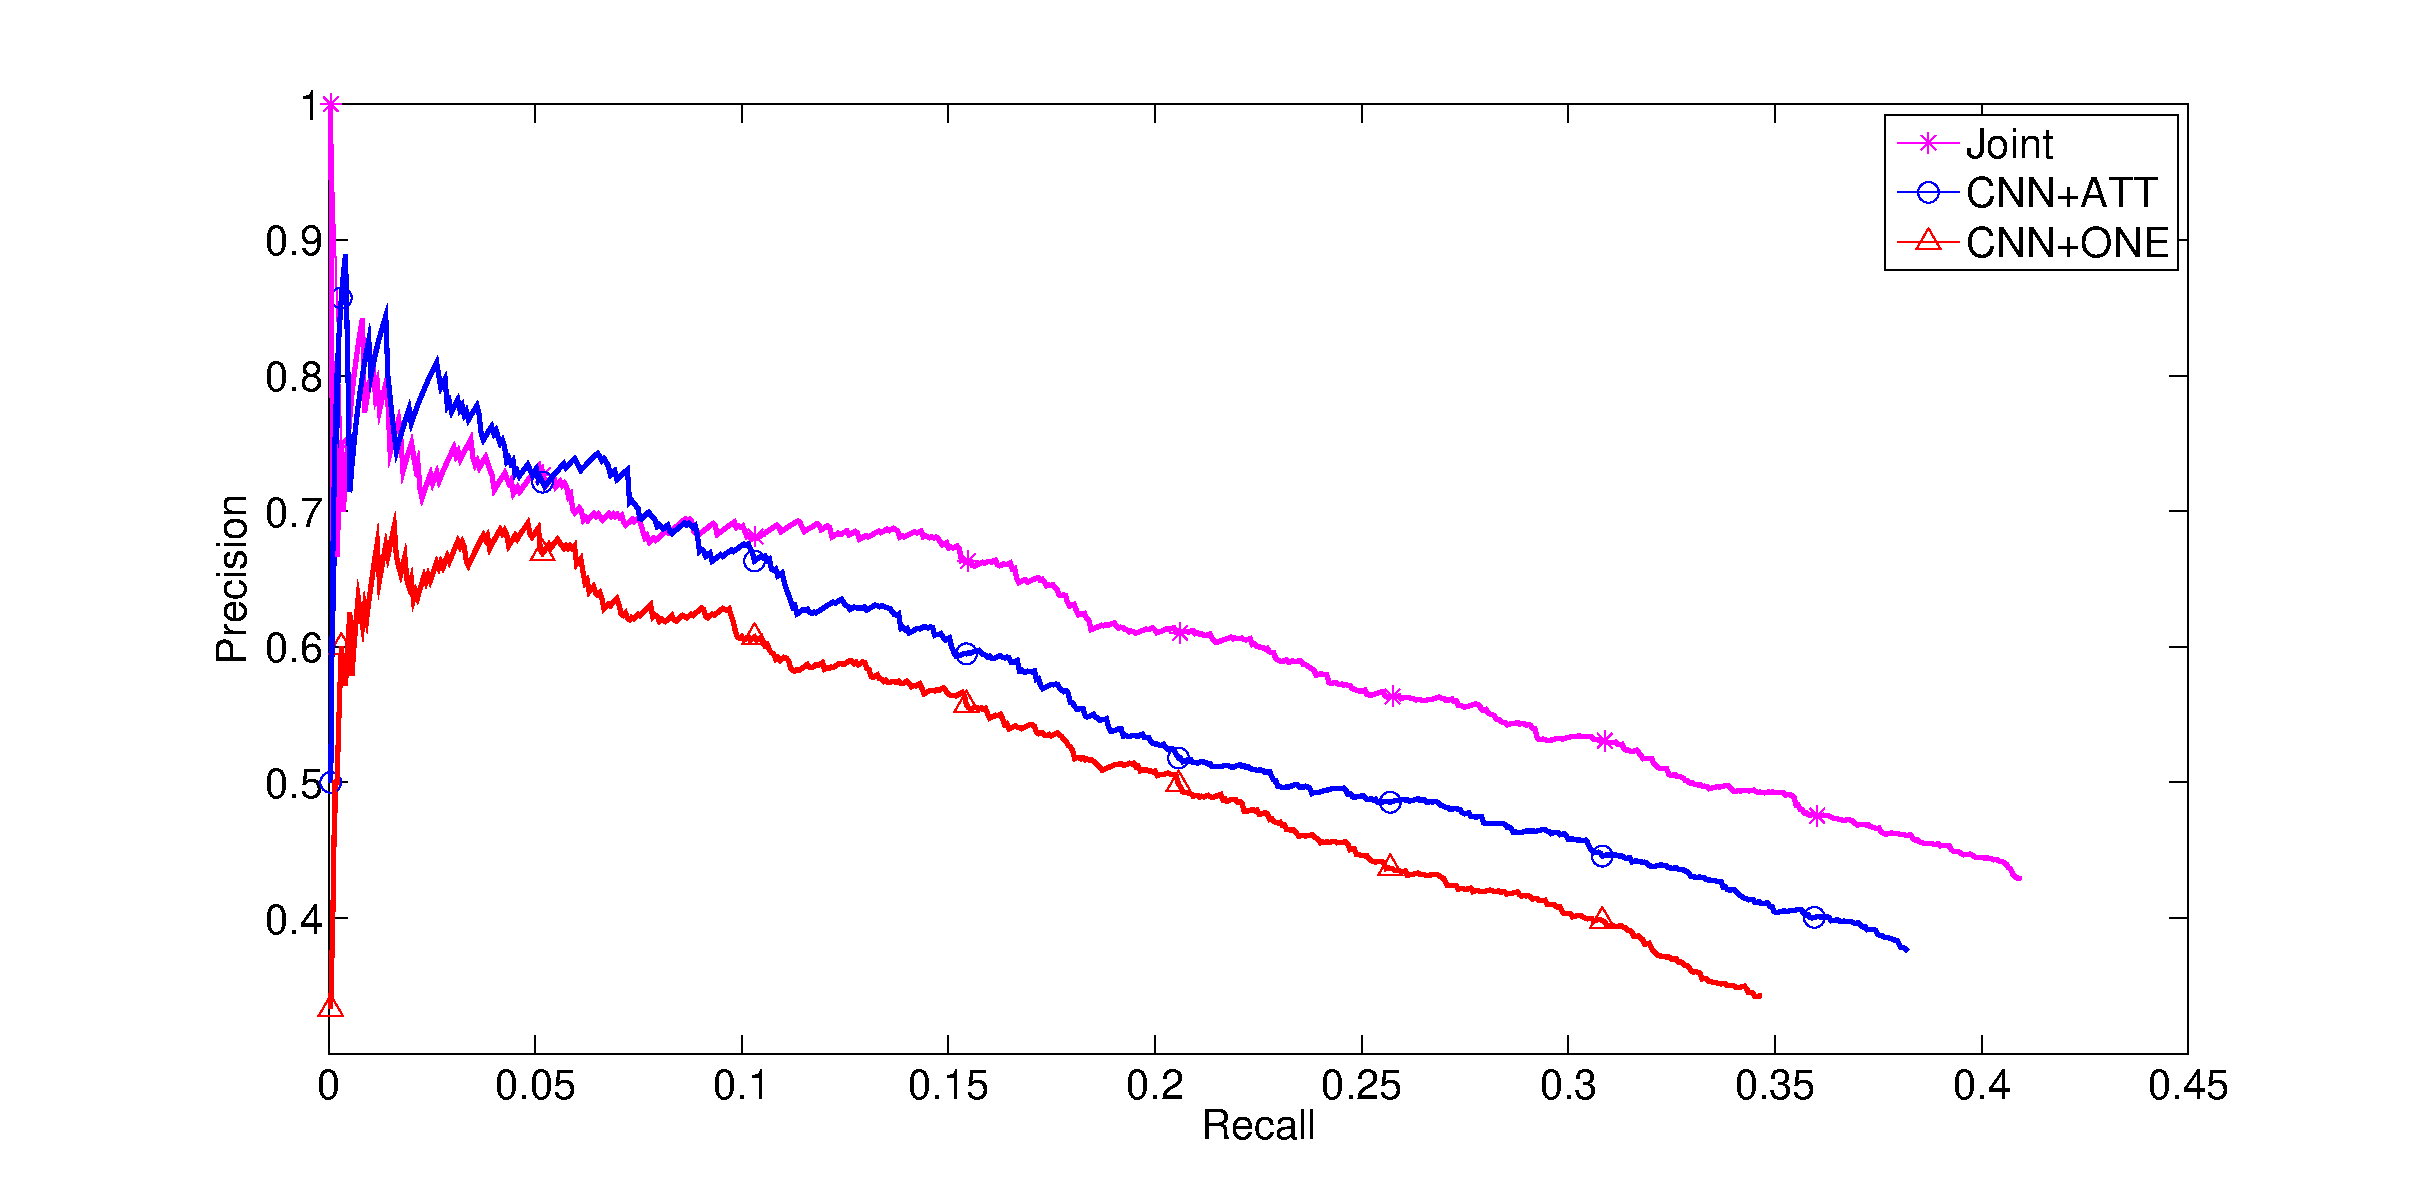
\includegraphics[width=1\columnwidth]{jointcnn.eps}
\caption{Aggregate precision/recall curves of joint learning model, CNN-ATT, CNN-ONE, MIML, MultiR and Mintz.}
\label{fig:jointcnn}
\end{figure} 




\begin{table*}[t]
\centering
\small
\begin{tabular}{|c|cccc|cccc|c|c|c|c|}
\hline
Metric            & \multicolumn{4}{c|}{Predicting Head} & \multicolumn{4}{c|}{Predicting Tail} & \multicolumn{2}{c|}{Overall} \\ \hline
      Category            & 1-to-1     & 1-to-N    & N-to-1    & N-to-N    & 1-to-1     & 1-to-N    & N-to-1    & N-to-N  & Triple Avg. & Relation Avg. \\ \hline

SE &35.6 &62.6 &17.2 &37.5 &34.9 &14.6 &68.3 &41.3 &39.8 & - \\ 
SME &35.1 &69.6 &19.9 &40.3 &32.7 &14.9 &76.0 &43.3 &41.3 & - \\ 
TransE            & 43.7       & 65.7      & 18.2      & 47.2      & 43.7       & 19.7      & 66.7      & 50.0    & 47.1 & - \\ 
TransH     & 66.8       & 87.6      & 30.2      & 64.5      & 65.5       & 39.8      & 83.3      & 67.2    & 64.4 & - \\ 
TransR     & 78.8       & 89.2      & 38.1      & 66.9      & 79.2       & 38.4      &\textbf{90.4}      & 72.1    & 68.7 & - \\ 
CTransR     & 81.5      & 89.0      & 36.4      & 71.2      & 80.8       & 38.6      &90.1      & 73.8    & 70.2 & - \\ 

TransD  &80.7  &85.8  &\textbf{47.1} &75.6  &80.0 &54.5 &80.7 &77.9  &74.2 &- \\ \hline


Prob-TransE      & 66.5       & 88.8      & 39.8      & 79.0      & 66.4       & 51.9      & 85.6      & 81.5    & 76.6 & 66.2 \\ 
Joint             & \textbf{82.7}& \textbf{89.1} &45.0 & \textbf{80.7}& \textbf{81.7}& \textbf{57.7}& 87.4&\textbf{82.8} & \textbf{78.7} & \textbf{79.1} \\ \hline
\end{tabular}
\caption{Evaluation results on entity prediction of head and tail entities (\%).}
\label{t:entity}
\end{table*}


\subsection{Results of Knowledge Graph Completion}

\subsubsection{Entity Prediction}

Entity prediction has also been used for evaluation in \cite{bordes2013translating,wang2014transh,lin2015learning,ji2015knowledge,he2015learning,xiao2015transg,ji2016knowledge}. More specifically, we need to predict the tail entity when given a triple $(h, r, ?)$ or predict the head entity when given a triple $(?, r ,t)$. In this task, for each missing entity, the system is asked to rank all candidate entities from the knowledge graph instead of only giving one best result. 

For each test triple $(h, r, t)$, we replace head and tail entities with all entities in FB15K ranked in descending order of distance scores calculated by $\lVert \textbf{h} + \textbf{r} - \textbf{t} \rVert$. The relational fact $(h, r, t)$ is expected to have smaller distance score than any other corrupted triples.

We follow previous works and use the proportion of correct entities in Top-10 ranked entities (Hits@10) as the evaluation metric. As mentioned in \cite{bordes2013translating}, a corrupted triple may also exist in knowledge graphs, which should not be considered as incorrect. Hence, before ranking, we filter out those corrupted triples that have appeared in FB15K.

The relations in knowledge graphs can be divided into four classes: 1-to-1, 1-to-N, N-to-1 and N-to-N relations, where a ``1-to-N'' relation indicates a head entity may correspond to multiple tail entities in knowledge graphs, and so on. For example, the relation (\emph{Country}, \texttt{PresidentOf}, \emph{Person}) is a typical ``1-to-N'' relation, because there used to be many presidents for a country in history. We report the average Hits@10 scores when predicting missing head entities and tail entities with respect to different classes of relations. We also report the overall performance by averaging the Hits@10 scores over triples and over relations.

Since the evaluation setting is identical, we simply report the results of SE, SME, TransE, TransH, TransR/CTransR, TransD from \cite{bordes2011learning,bordes2012joint,bordes2013translating,wang2014transh,lin2015learning,ji2015knowledge}. The evaluation results on entity prediction is shown in Table \ref{t:entity}. The model for knowledge representation without joint learning in our framework is named as ``Prob-TransE''. From Table \ref{t:entity} we observe that:

(1) The joint model almost achieves improvements under four classes of relations when predicting head and tail entities. This indicates the improvement of joint learning for knowledge representations is consistent and robust. 

(2) The improvements on ``1-to-1'', ``1-to-N'' and ``N-to-1'' relations are much more significant as compared to those on ``N-to-N''. This indicates that our joint model is more effective to embed textual relations for those deterministic relations.

(3) Our joint model achieves improvement of more than $13\%$ than Prob-TransE when averaging over relations. This indicates that, our joint model can take advantages of plain texts and greatly improve representation power in relation-level. In FB15K, the relation numbers in different relation classes are comparable, but more than $80\%$ triples are instances of ``N-to-N'' relations. Since the improvement of the joint model on ``N-to-N'' relations is not as remarkable as on other relation classes, hence the overall superiority of our joint model seems not so notable when averaging over triples as compared to averaging over relations.

\subsubsection{Results of Relation Prediction}
The task aims to predict the missing relation between two entities based on their embeddings. More specifically, we need to predict the relation when given a triple $(h, ?, t)$. In this task, for each missing relation, the system is asked to find one best result, according to similarity scores calculated by $\lVert \textbf{h} + \textbf{r} - \textbf{t} \rVert$.
Because the number of relations is much smaller as compared with the number of entities, we use the accuracy of Top-1 ranked relations as the evaluation metric. Since some entity pairs may have more than one relation, we also filter out those triples with corrupted relations appeared in KGs. We report the overall evaluation results as well as those in different relation classes.

\begin{table}[htb]
\centering
\small 
\begin{tabular}{|c|c|c|c|c|c|}
\hline
Tasks             & \multicolumn{5}{c|}{Relation Prediction}                      \\ \hline
Category & 1-to-1     & 1-to-N     & N-to-1     & N-to-N     & All           \\ \hline
Prob-TransE       & 24.1       & 83.0       & 80.4       & 92.5       & 87.2          \\ \hline
Joint             & \textbf{40.9} & \textbf{89.4} & \textbf{87.1} & \textbf{94.6} & \textbf{91.6} \\ \hline
\end{tabular}
\caption{Evaluation results on relation prediction (\%).}
\label{t:relation}
\end{table}

The evaluation results are shown in Table \ref{t:relation}. From Table \ref{t:relation} we observe that, our joint model outperforms Prob-TransE consistently in different classes of relations. The joint model also achieves more significant improvements on ``1-to-1'', ``1-to-N'' and ``N-to-1'' relations. The observations are compatible with those on entity prediction.


\section{Conclusion and Future Work}

In this paper, we propose a model for joint representation learning of KGs and text. Our joint model embeds entities, relations and words within a unified continuous latent space. More specifically, we adopt CNN with the knowledge-based attention to encode textual relations for joint learning of relation embeddings. In experiments, we evaluate our model on both RE and KGC. Experiment results show that the joint learning model can effectively perform representation learning for both the KG and text, and obtain more discriminative embeddings for knowledge acquisition. In the future, we will explore the following research directions: 

(1) We will explore to adopt RNN or LSTM for encoding textual relations in an efficient manner.

(2) Our joint model is capable to incorporate other knowledge representation models besides TransE, such as TransH, TransR and so on. In future we will explore their capability in our joint model. 

(3) We will also take more rich information in our joint model, such as relation paths in KGs, and the textual relations represented by more than one sentence in a paragraph or document.

\bibliography{acl2017}
\bibliographystyle{acl_natbib}

\end{document}
